\section{VLBI Measurements and Data Products}
\label{sec:meas}



\begin{figure*}[h!]
	\vspace{-.3in}
	\begin{center}
		%\hspace*{-0.5cm}
		\begin{tabular}{  c  c   }
			%\hline
			\large{\textsf{Visibility Amplitude}}   &\large{\textsf{Closure Phase}}      \\ 
			%\large{\textsf{Single Frame}} &
			\small{\textsf{ALMA-SPT Baseline}}   &\small{\textsf{ALMA-SPT-PV Triangle}}      \\ 
			%{{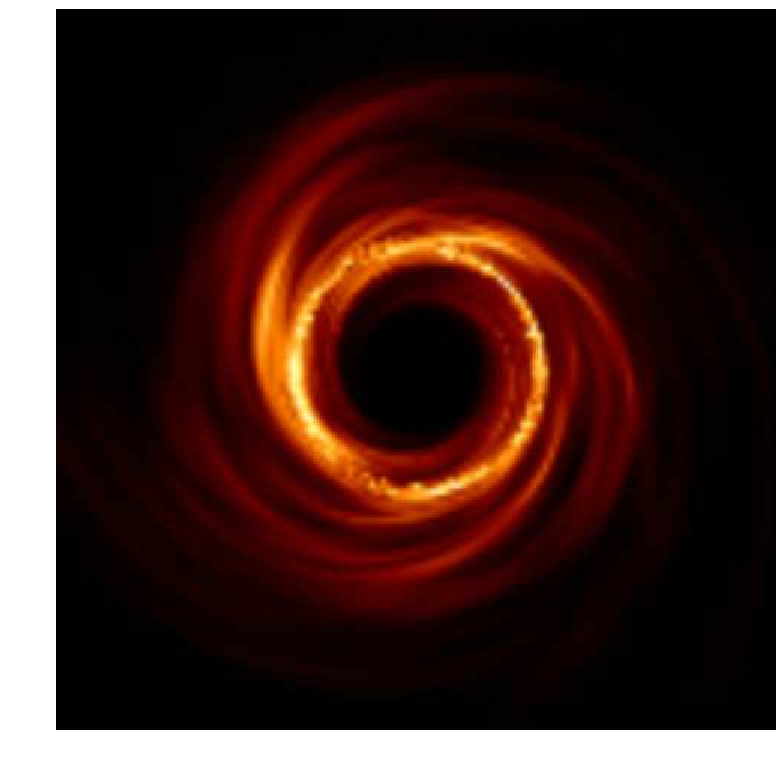
\includegraphics[height=.15\linewidth]{/Users/klbouman/Research/vlbi_imaging/papers/starwarps/9240887pjjjtcdggvxt/figures/compare_var2static/hotakaframe_noaxis.pdf}} } &
			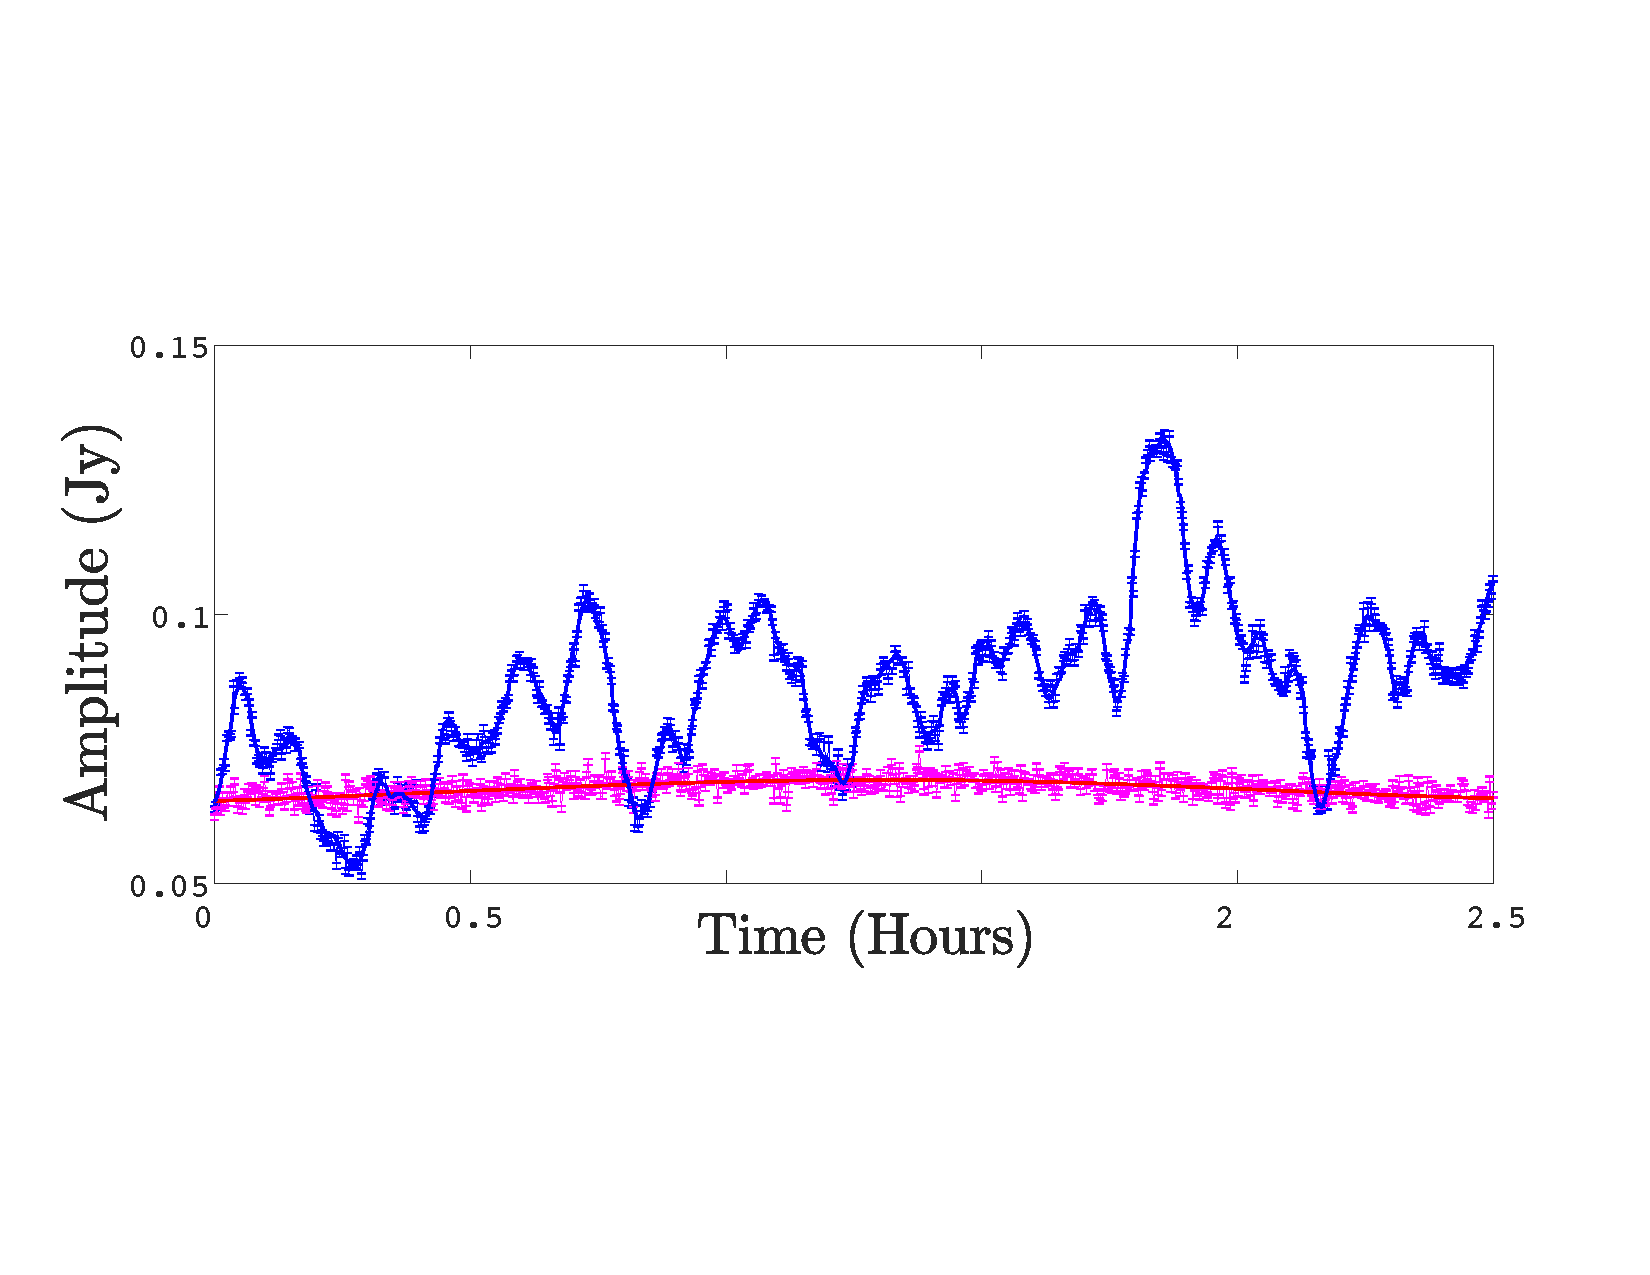
\includegraphics[width=.47\linewidth]{figures/compare_var2static/visamplitudes_notitle_editted.pdf} &
			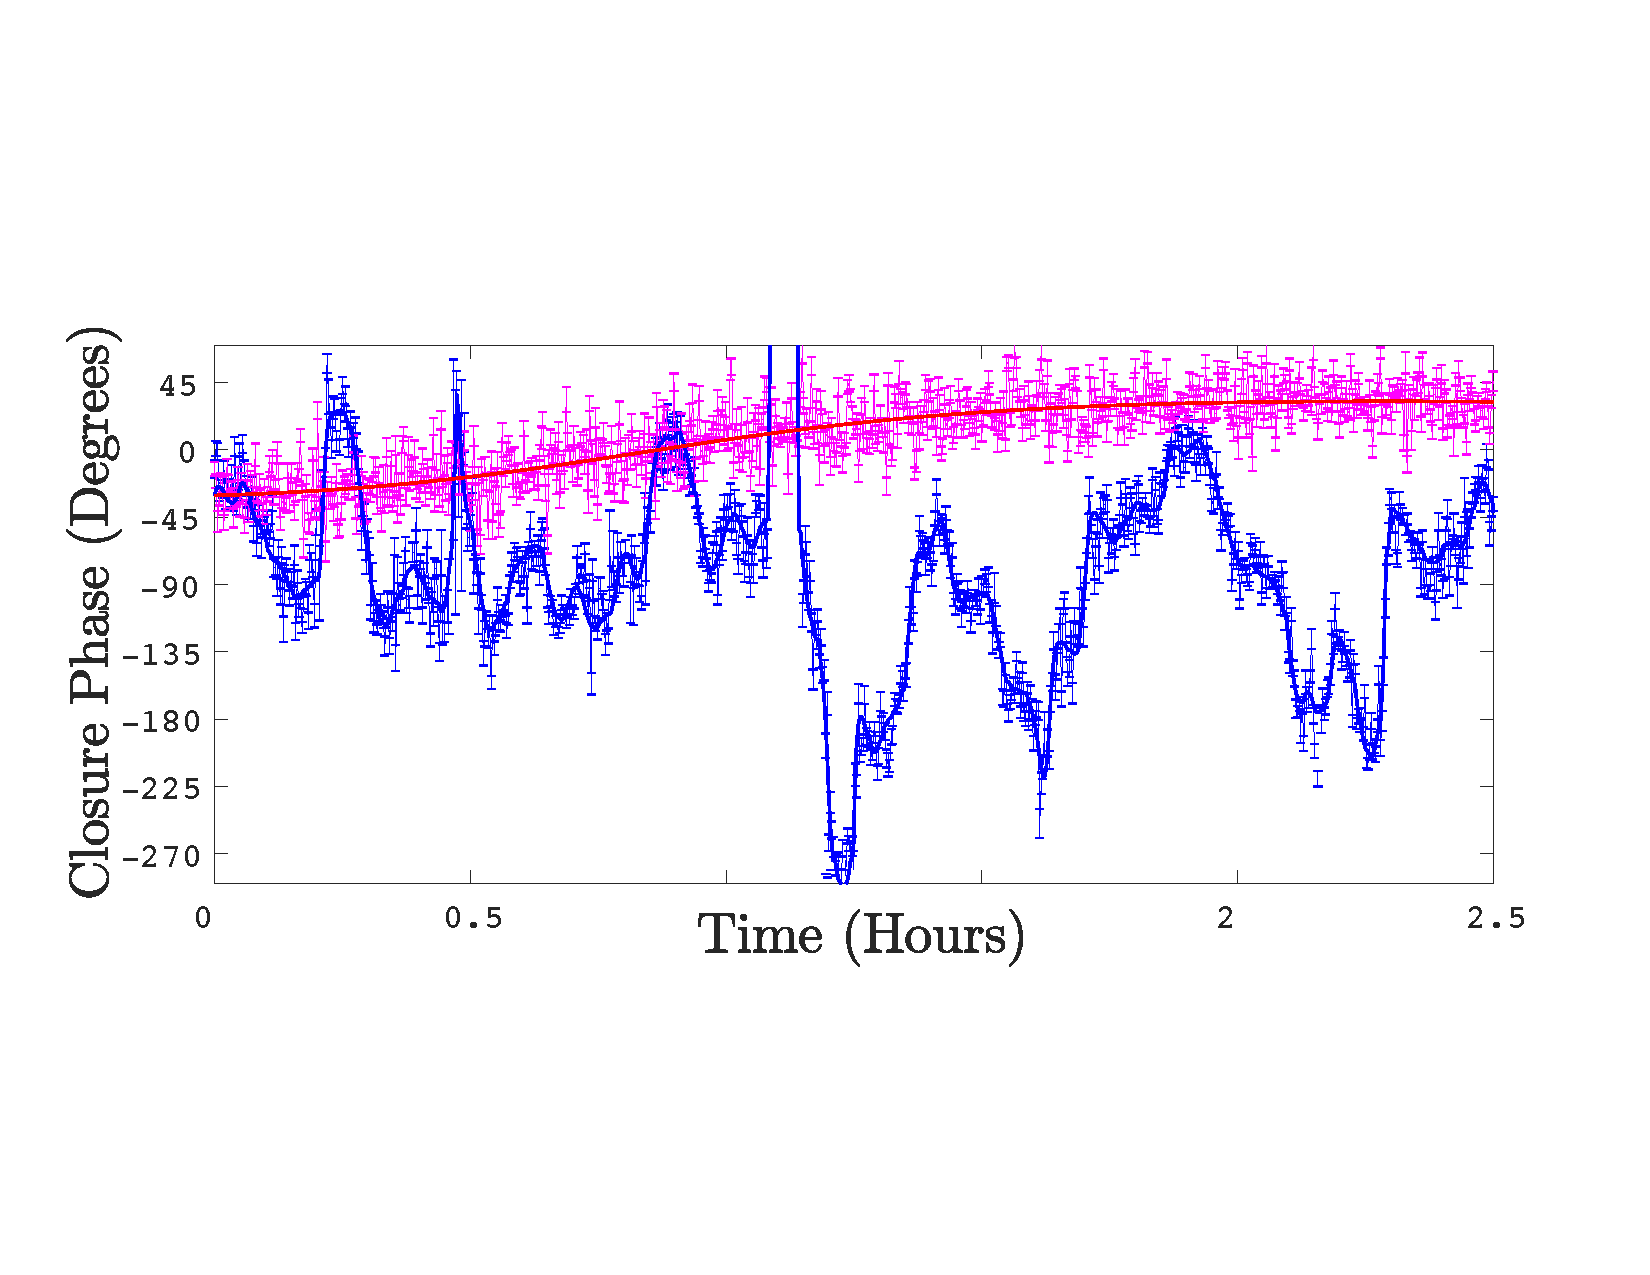
\includegraphics[width=.47\linewidth]{figures/compare_var2static/closurephase_notitle_editted.pdf} 
			\\
		\end{tabular}
		\caption{{\bf Simulated data under a static vs. varying source:} Contrasting of data observed from a static emission region (magenta) to that of a varying emission region (blue) over the course of 2.5 hours. Although both sequences start with the same image, the visibility amplitude and closure phase both begin to deviate from the static image very quickly. The ideal observation for the static and time-varying source is shown by the solid red and blue lines, respectively. We also show sample measurements with their respective error bars in the same colors. This data is simulated at a sampling interval of 11 seconds using the EHT2017 array from the frames in Video 3 presented in Section~\ref{sec:results}. This figure shows 1 of the ${\nmeas \choose 2}$ possible visibility amplitudes and 1 of ${\nmeas \choose 3}$ possible closure phases (phase of the bispectrum). }
		\label{fig:amplandphase}
	\end{center}
	\vspace{-.2in}
\end{figure*}

%KATIE REMOVED THIS PARAGRAPH
A single-dish telescope is diffraction limited, with an angular resolution dictated by the ratio of wavelength to dish diameter~\cite{TMS}. This governing law limits the highest achievable angular resolution of traditional single-dish telescopes. For example, past observations and simulations suggest that the emission surrounding SgrA* subtends approximately $2.5 \times 10^{-10}$ radians, or $50$ $\mu$-arcseconds~\cite{Doeleman_2008}. Imaging this emission region at $1.3$ mm wavelength would require an impossibly large single-dish telescope with a $13,000$ km diameter. However, simultaneously collecting data from an array of telescopes, called an interferometer, allows us to overcome the single-dish diffraction limit, and create a virtual telescope as large as the maximum distance between telescopes in the array. When these telescopes are distributed globally, using separate clocks and recording systems, this technique is referred to as Very Long Baseline Interferometry (VLBI)~\cite{TMS}. 


An interferometer consists of $\ntele$ telescopes simultaneously observing and recording time-stamped data-streams of light traveling from a common source~\cite{TMS}.
%An interferometer consists of $\ntele$ telescopes simultaneously observing a common source. Each telescope records a time-stamped data-stream of the intensity of light traveling from the astronomical emission.
From these measurements a number of different {\it data products} can be computed. 
% This data 
% is a function of the source image's flux (brightness) distribution, and thus is used to constrain image reconstruction. 
%Therefore, for an evolving source, these data products often change erratically over short periods of time (Figure~\ref{fig:amplandphase}).
Depending on the imaging technique and the quality of the measurements, different data products may be used. In this section we review a number of common data products used in VLBI imaging, and throughout this paper. 

%We review the different types of data products, and how we BLAH BLAH BLAH. 

%\begin{align}
%f(x): \Re^{ M^2 \times 1} \rightarrow \Re^{ | y | \times 1 }
%\end{align}

\vspace{-.2in}
\subsection{Visibilities }
\label{sec:vis}


%An interferometer consists of $\ntele$ telescopes simultaneously observing a common source. 
The time-averaged cross-correlation of the recorded scalar electric fields at two telescopes, called a {\it visibility}, provides information about the spatial structure of the observed source\footnote{Although the particular length of time-averaging varies per experiment, for the EHT data is averaged over sub-second intervals before additional coherent averaging is done to increase SNR (on an order of 5-100 seconds).}. Formally, the van Cittert-Zernike theorem states that a visibility, $\vis(I, u,v)$ is related to the ideal source image $I(\xpos, \ypos)$ through a Fourier transform: 
\begin{align}
\vis(I, u,v) \approx \int_{\xpos} \int_{\ypos} e^{-i2 \pi (u\xpos + v \ypos) } I(\xpos, \ypos) d\xpos d\ypos
\label{eq:vcz}
\end{align}
\noindent{where $(\xpos,\ypos)$ is the angular sky coordinate in radians, and $(u,v)$ is the dimensionless baseline vector between two telescopes, measured in wavelengths and orthogonal to the source direction~\cite{TMS}. Note that each visibility is a complex value with both an amplitude and a phase. As each visibility is calculated from a pair of telescopes, for a $\ntele$ telescope array we can obtain up to $\frac{\ntele (\ntele - 1)}{2}$ visibility measurements at a single instant in time. The image spatial frequency sampled by a visibility is related to the distance between the telescopes; telescopes that are father apart inform us about higher spatial frequencies of the underlying image.}
For radio wavelengths, the thermal noise appearing on perfectly calibrated visibilities is 
circularly Gaussian in the real-imaginary plane\footnote{In practice, the thermal noise is calculated from first principles using measured SEFD values at each telescope (see Eq~\ref{eq:thermal}) or estimated empirically. }~\cite{taylor1999synthesis}.


%Note, that the frequency of a visibility is related to the distance between the telescopes; and the resolution of the underlying image sampled by the interferometer is governed by the maximum distance between telescopes in the array. 


%are located the finer the structure they inform on for the source emission. 

%\subsection{Earth Rotation Synthesis}


\vspace{-.1in}
\subsection{Bispectrum and Closure Phases }
\label{sec:bispec}

%For instance, at these short wavelengths, rapidly varying inhomogeneities in the atmosphere introduce additional measurement errors

The van Cittert-Zernike theorem (Equation~\ref{eq:vcz}) is derived under the assumption that light is moving through a vacuum. 
%In all equations and derivations above it was assumed that light was moving through a vacuum. 
However, in reality, inhomogeneity in the Earth's atmosphere causes the light to move at different velocities towards each telescope. At short observing wavelengths, this propagation delay has a large effect on the phase of measurements, and renders the absolute visibility phase unusable for image reconstruction~\cite{monnier2013radio}. Although absolute phase measurements cannot be used, a property called phase closure allows us to still obtain some information from these phases. 

Consider three telescopes, denoted by $i, j$, and $k$, observing the same source. From each pair of telescopes we compute a visibility: $\vis_{i,j}, \vis_{j,k}, \vis_{k,i}$. Rapidly changing atmospheric propagation delays, resulting in phase errors of $\phi_i$ and $\phi_j$ to telescopes $i$ and $j$ respectively, will cause error in the visibility's phase: 
\begin{equation} \vis_{i,j}^{\mbox{\tiny{meas}}} = e^{i(\phi_i - \phi_j)}\vis_{i,j}^{\mbox{\tiny{ideal}}}. 
\end{equation}
\noindent{However, by multiplying the visibilities from 3 different telescopes in a closed loop, we obtain a term that is invariant to the atmosphere (Equation~\ref{eq:phaseclosure})~\cite{jennison}.   }
\begin{align}  
\notag \vis^{\mbox{\tiny{meas}}}_{i,j}\vis^{\mbox{\tiny{meas}}}_{j,k}\vis^{\mbox{\tiny{meas}}}_{k,i} &= e^{i(\phi_i-\phi_j)}\vis^{\mbox{\tiny{ideal}}}_{i,j}e^{i(\phi_j-\phi_k)}\vis^{\mbox{\tiny{ideal}}}_{j,k}e^{i(\phi_k-\phi_i)}\vis^{\mbox{\tiny{ideal}}}_{k,i} \\
%& = e^{i(\phi_i-\phi_j+\phi_j-\phi_k + \phi_k-\phi_i)}\vis^{\mbox{\tiny{true}}}_{i,j}\vis^{\mbox{\tiny{true}}}_{j,k}\vis^{\mbox{\tiny{true}}}_{k,i} \\
&=\vis^{\mbox{\tiny{ideal}}}_{i,j}\vis^{\mbox{\tiny{ideal}}}_{j,k}\vis^{\mbox{\tiny{ideal}}}_{k,i}. %= B_{i,j,k}
\label{eq:phaseclosure}
 \end{align}

We refer to the multiplication of these three complex visibilities in a closed loop 
%$( B_{i,j,k} = \vis^{\mbox{\tiny{true}}}_{i,j}\vis^{\mbox{\tiny{true}}}_{j,k}\vis^{\mbox{\tiny{true}}}_{k,i} ) $ 
as the {\it bispectrum}, and the phase of the bispectrum %$\angle{ \bispec }$ 
as the {\it closure phase}.
Although these data products are invariant to atmospheric noise, they come at the cost of having a fewer number of independent data points - only $\frac{(\ntele-1)(\ntele-2)}{2}$ compared to  $\frac{\ntele(\ntele-1)}{2}$ independent visibilities. Additionally, when using these data products, information related to the absolute location of the source is lost. 

As each bispectrum (Eq.~\ref{eq:phaseclosure}) is the multiplication of three visibilities with Gaussian noise, its noise is not Gaussian. 
Although the noise cannot be fully expressed simply with a covariance matrix, we follow~\cite{bouman2016computational} and approximate the bispectrum's distribution as Gaussian with a best-fit covariance matrix.
%Although the bispectrum noise cannot be expressed simply with a covariance matrix, the noise can be approximated with a best-fit covariance~\cite{bouman2016computational}. 
Refer to the supplemental material for a derivation of this approximation. 

%As each bispectrum is the multiplication of three Gaussian random variables, it is not itself a Gaussian random variable. Although the noise on each bispectrum cannot be expressed simply as a covariance, we can approximate the noise by finding the best fit covariance using the method described in BLAH.

%Recall that each pair of telescopes at a given time is associated with a single $(u,v)$ vector, and that 3 telescopes correspond with $(u,v)$ vectors that form a closed triangle. Therefore, we write this term as:

%\begin{align}
%\bispec(I, u_1, v_1, u_2, v_2) = \vis(I, u_1, v_1) \vis(I, u_2, v_2) \vis (I, u_1 - u_2, v_1 - v_2)
%\end{align}

 
 
\vspace{-.1in}
\subsection{Visibility Amplitudes }
\label{sec:visamp}

%In addition to causing rapid fluctuation of the phase, atmospheric inhomogeneity also introduces fluctuations on the visibility amplitude. 


%Although atmospheric inhomogeneity causes substantial phase errors in the complex visibility, with careful calibration, the visibility's amplitude can be much more accurately estimated. 



%Constraining image reconstruction using the bispectrum's phase closure property is essential in recovering the image's phase. However, in addition to 

Bispectrum measurements not only entangle the phase, but also the amplitudes of the three corresponding spatial frequency components. 
Although atmospheric inhomogeneity causes substantial phase errors in each complex visibility, with careful calibration the amplitude of the visibility can be well estimated. Thus, we have found that during image reconstruction it is quite helpful to additionally constrain the visibility amplitude in addition to the bispectrum or closure phase. Empirically we have found this to be especially important when reconstructing an image with a large field of view. 
%The {\it visibility amplitude} of visibility $\vis(I,u,v)$ is defined by 
%\begin{align}
%| \vis(I,u,v) | = \sqrt{\Re \left[ \vis(I,u,v)\right]^2 + \Im \left[ \vis(I,u,v)\right]^2}
%\end{align}
%\noindent{where $\Re[x]$ and $\Im[x]$ extract the real and imaginary portion of $x$, respectively.}
As thermal noise is isotropic in the real-imaginary plane, a perfectly gain-calibrated visibility amplitude has the same standard deviation of noise as a perfectly calibrated complex visibility \cite{TMS}. 
%Although not used in this work, a convex solution that recovers an image solely from the squared amplitude of the visibilities is discussed in~\cite{demanet}.



